\section{Summary}
\label{sec:evaluation-summary}

The results from the developer survey (see Section~\ref{sec:evaluation:developer-survey}) have shown that the resulting simple file-based repository design is easy to work with and could potentially simplify repository management tasks. Furthermore, the results also indicate that a simple file-based repository design would have little impact on the extensibility of an application built on top of such a repository design.

The implementation case study collections outlined in Section~\ref{ch:case-studies} serve as proof that the proposed approach is effective; the Bleek and Lloyd\index{Bleek and Lloyd} case study (see Section~\ref{sec:case-studies:bleek-and-lloyd}) in particular serves as proof that system functionalities and features of existing services based on conventional storage solutions can be replicated using a simple file-based digital object store with little adverse effect.

The scalability performance experiments yielded results that strongly indicate that the performance would be within generally acceptable limits for medium-sized collections, as evidenced in the Kiviat\index{Kiviat} plot shown in Figure~\ref{fig:experimentation:performance:summary:kiviat}. Figure~\ref{fig:experimentation:performance:summary:kiviat} also indicates that ingestion\index{Ingestion} performance is significantly better than the other services. In addition, the performance degradation for all other services occurs for collections with larger than \num{12800} objects. It was further shown that performance degradation of operations such as information discovery and OAI-PMH\index{OAI-PMH} associated services are largely as a result of parsing, a problem that can easily be remedied through the use of an index. 

Finally, it was shown that the superior performance results from the comparative experiments done with DSpace\index{DSpace} are attributed to the external index\index{Index} service---Apache Solr\index{Apache!Solr} and Lucene\index{Lucene}---integrated with DSpace\index{DSpace} to facilitate fast search. However, it was shown in the indexing experiments (see Section~\ref{sec:evaluation:performance:indexing}) that integration of such an external search service could easily be performed using the proposed approach.

\begin{figure}
 \centering
 \framebox[\textwidth]{%
% Created by tikzDevice version 0.6.2-92-0ad2792 on 2013-03-28 12:32:35
% !TEX encoding = UTF-8 Unicode
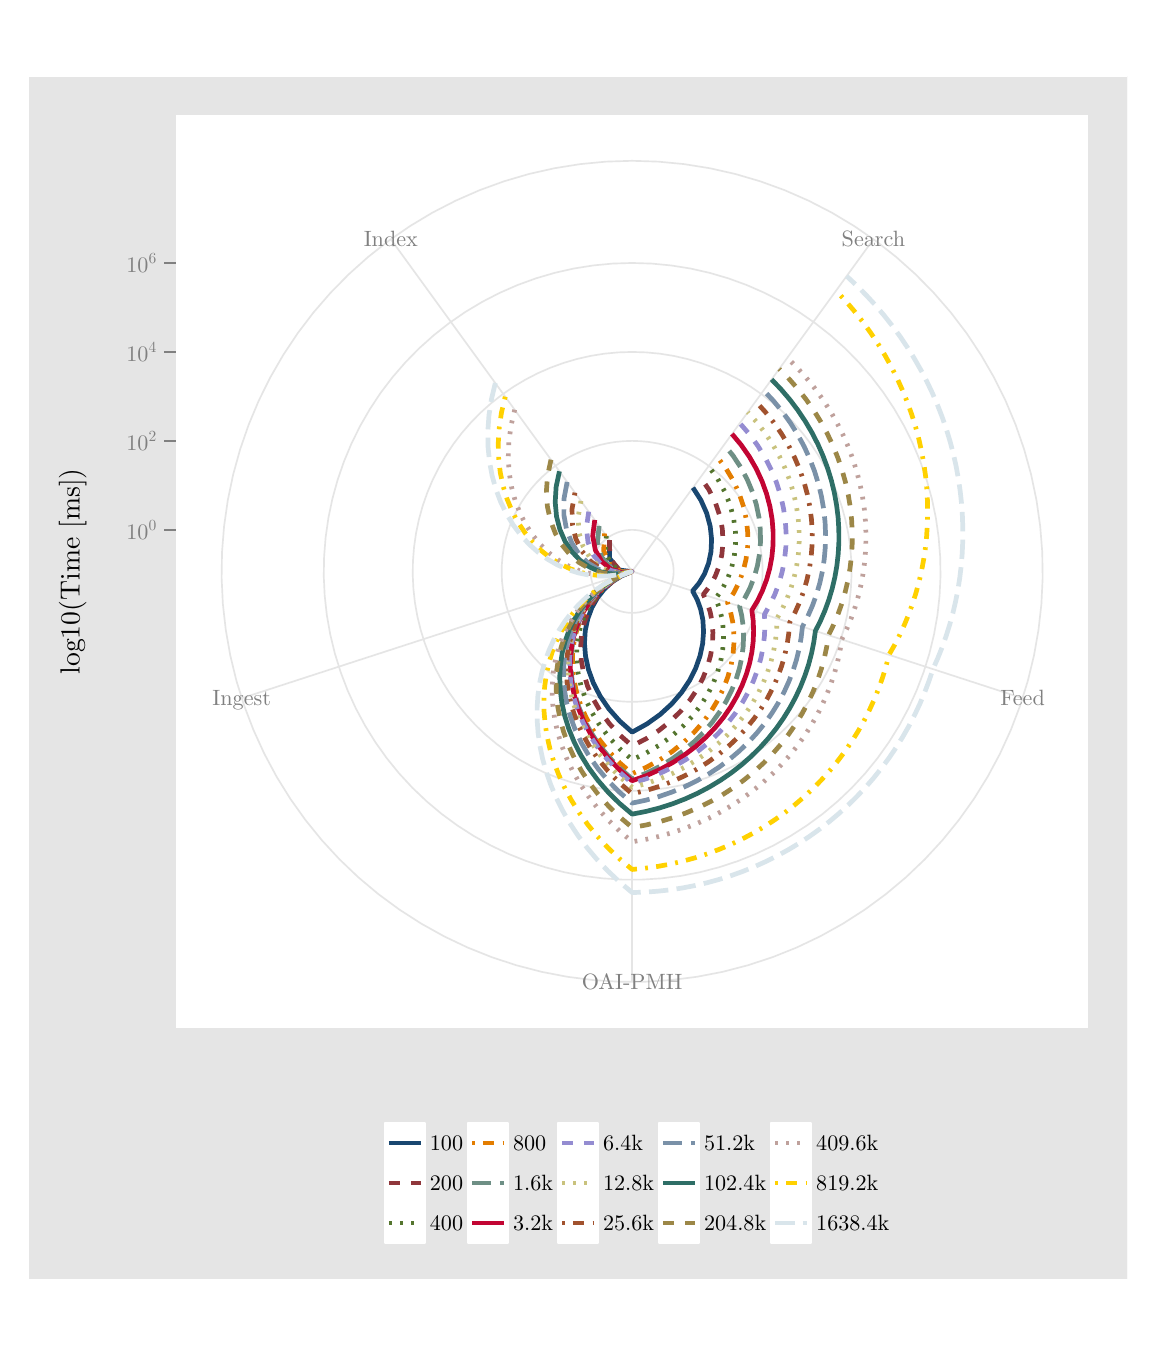
\begin{tikzpicture}[x=1pt,y=1pt]
\definecolor[named]{fillColor}{rgb}{1.00,1.00,1.00}
\path[use as bounding box,fill=fillColor,fill opacity=0.00] (0,0) rectangle (397.48,469.75);
\begin{scope}
\path[clip] (  0.00, 17.41) rectangle (397.48,452.35);
\definecolor[named]{drawColor}{rgb}{1.00,1.00,1.00}
\definecolor[named]{fillColor}{rgb}{0.90,0.90,0.90}

\path[draw=drawColor,line width= 0.6pt,line join=round,line cap=round,fill=fillColor] (  0.00, 17.41) rectangle (397.48,452.35);
\end{scope}
\begin{scope}
\path[clip] ( 53.58,108.44) rectangle (383.26,438.12);
\definecolor[named]{fillColor}{rgb}{1.00,1.00,1.00}

\path[fill=fillColor] ( 53.58,108.44) rectangle (383.26,438.12);
\definecolor[named]{drawColor}{rgb}{0.90,0.90,0.90}

\path[draw=drawColor,line width= 0.6pt,line join=round] (218.42,273.28) --
	(131.22,393.30);

\path[draw=drawColor,line width= 0.6pt,line join=round] (218.42,273.28) --
	( 77.33,227.44);

\path[draw=drawColor,line width= 0.6pt,line join=round] (218.42,273.28) --
	(218.42,124.93);

\path[draw=drawColor,line width= 0.6pt,line join=round] (218.42,273.28) --
	(359.51,227.44);

\path[draw=drawColor,line width= 0.6pt,line join=round] (218.42,273.28) --
	(305.62,393.30);

\path[draw=drawColor,line width= 0.6pt,line join=round] (218.42,288.28) --
	(219.37,288.25) --
	(220.32,288.16) --
	(221.26,288.01) --
	(222.19,287.80) --
	(223.10,287.53) --
	(223.99,287.20) --
	(224.87,286.82) --
	(225.71,286.39) --
	(226.53,285.90) --
	(227.31,285.36) --
	(228.06,284.77) --
	(228.77,284.13) --
	(229.44,283.46) --
	(230.06,282.74) --
	(230.64,281.98) --
	(231.16,281.19) --
	(231.64,280.36) --
	(232.06,279.51) --
	(232.43,278.63) --
	(232.74,277.73) --
	(232.99,276.82) --
	(233.19,275.89) --
	(233.32,274.94) --
	(233.40,273.99) --
	(233.41,273.04) --
	(233.37,272.09) --
	(233.26,271.15) --
	(233.10,270.21) --
	(232.87,269.29) --
	(232.59,268.38) --
	(232.25,267.49) --
	(231.86,266.62) --
	(231.41,265.78) --
	(230.91,264.97) --
	(230.35,264.20) --
	(229.75,263.46) --
	(229.11,262.76) --
	(228.42,262.11) --
	(227.69,261.49) --
	(226.92,260.93) --
	(226.12,260.41) --
	(225.29,259.95) --
	(224.43,259.54) --
	(223.55,259.19) --
	(222.65,258.89) --
	(221.72,258.65) --
	(220.79,258.47) --
	(219.85,258.35) --
	(218.90,258.29) --
	(217.94,258.29) --
	(217.00,258.35) --
	(216.05,258.47) --
	(215.12,258.65) --
	(214.20,258.89) --
	(213.29,259.19) --
	(212.41,259.54) --
	(211.55,259.95) --
	(210.72,260.41) --
	(209.92,260.93) --
	(209.15,261.49) --
	(208.42,262.11) --
	(207.73,262.76) --
	(207.09,263.46) --
	(206.49,264.20) --
	(205.94,264.97) --
	(205.43,265.78) --
	(204.98,266.62) --
	(204.59,267.49) --
	(204.25,268.38) --
	(203.97,269.29) --
	(203.74,270.21) --
	(203.58,271.15) --
	(203.47,272.09) --
	(203.43,273.04) --
	(203.44,273.99) --
	(203.52,274.94) --
	(203.65,275.89) --
	(203.85,276.82) --
	(204.10,277.73) --
	(204.41,278.63) --
	(204.78,279.51) --
	(205.20,280.36) --
	(205.68,281.19) --
	(206.21,281.98) --
	(206.78,282.74) --
	(207.40,283.46) --
	(208.07,284.13) --
	(208.78,284.77) --
	(209.53,285.36) --
	(210.31,285.90) --
	(211.13,286.39) --
	(211.98,286.82) --
	(212.85,287.20) --
	(213.74,287.53) --
	(214.65,287.80) --
	(215.58,288.01) --
	(216.52,288.16) --
	(217.47,288.25) --
	(218.42,288.28);

\path[draw=drawColor,line width= 0.6pt,line join=round] (218.42,320.43) --
	(221.41,320.33) --
	(224.39,320.05) --
	(227.34,319.57) --
	(230.26,318.91) --
	(233.13,318.07) --
	(235.94,317.05) --
	(238.68,315.85) --
	(241.34,314.48) --
	(243.91,312.94) --
	(246.37,311.24) --
	(248.72,309.40) --
	(250.95,307.40) --
	(253.05,305.27) --
	(255.01,303.01) --
	(256.82,300.63) --
	(258.48,298.14) --
	(259.98,295.55) --
	(261.30,292.87) --
	(262.46,290.11) --
	(263.44,287.28) --
	(264.24,284.40) --
	(264.85,281.47) --
	(265.27,278.51) --
	(265.51,275.52) --
	(265.56,272.53) --
	(265.42,269.54) --
	(265.08,266.57) --
	(264.57,263.63) --
	(263.86,260.72) --
	(262.97,257.86) --
	(261.90,255.07) --
	(260.66,252.35) --
	(259.25,249.71) --
	(257.67,247.17) --
	(255.94,244.73) --
	(254.05,242.41) --
	(252.02,240.21) --
	(249.85,238.15) --
	(247.56,236.22) --
	(245.15,234.45) --
	(242.64,232.83) --
	(240.02,231.38) --
	(237.32,230.09) --
	(234.54,228.98) --
	(231.70,228.05) --
	(228.81,227.30) --
	(225.87,226.73) --
	(222.90,226.35) --
	(219.92,226.16) --
	(216.92,226.16) --
	(213.94,226.35) --
	(210.97,226.73) --
	(208.03,227.30) --
	(205.14,228.05) --
	(202.30,228.98) --
	(199.52,230.09) --
	(196.82,231.38) --
	(194.20,232.83) --
	(191.69,234.45) --
	(189.28,236.22) --
	(186.99,238.15) --
	(184.82,240.21) --
	(182.79,242.41) --
	(180.91,244.73) --
	(179.17,247.17) --
	(177.59,249.71) --
	(176.18,252.35) --
	(174.94,255.07) --
	(173.87,257.86) --
	(172.98,260.72) --
	(172.28,263.63) --
	(171.76,266.57) --
	(171.42,269.54) --
	(171.28,272.53) --
	(171.33,275.52) --
	(171.57,278.51) --
	(171.99,281.47) --
	(172.61,284.40) --
	(173.40,287.28) --
	(174.38,290.11) --
	(175.54,292.87) --
	(176.87,295.55) --
	(178.36,298.14) --
	(180.02,300.63) --
	(181.83,303.01) --
	(183.79,305.27) --
	(185.89,307.40) --
	(188.12,309.40) --
	(190.47,311.24) --
	(192.93,312.94) --
	(195.50,314.48) --
	(198.16,315.85) --
	(200.90,317.05) --
	(203.71,318.07) --
	(206.58,318.91) --
	(209.50,319.57) --
	(212.45,320.05) --
	(215.43,320.33) --
	(218.42,320.43);

\path[draw=drawColor,line width= 0.6pt,line join=round] (218.42,352.57) --
	(223.45,352.41) --
	(228.46,351.94) --
	(233.43,351.14) --
	(238.33,350.03) --
	(243.16,348.61) --
	(247.89,346.89) --
	(252.50,344.88) --
	(256.97,342.57) --
	(261.29,339.99) --
	(265.43,337.13) --
	(269.39,334.02) --
	(273.14,330.67) --
	(276.67,327.08) --
	(279.96,323.28) --
	(283.01,319.28) --
	(285.80,315.09) --
	(288.31,310.73) --
	(290.55,306.22) --
	(292.49,301.58) --
	(294.14,296.82) --
	(295.48,291.97) --
	(296.51,287.05) --
	(297.22,282.07) --
	(297.62,277.05) --
	(297.70,272.02) --
	(297.46,267.00) --
	(296.91,262.00) --
	(296.03,257.04) --
	(294.85,252.15) --
	(293.35,247.35) --
	(291.56,242.65) --
	(289.47,238.07) --
	(287.09,233.64) --
	(284.44,229.36) --
	(281.52,225.26) --
	(278.35,221.36) --
	(274.93,217.66) --
	(271.29,214.19) --
	(267.44,210.95) --
	(263.38,207.97) --
	(259.15,205.25) --
	(254.75,202.80) --
	(250.21,200.64) --
	(245.54,198.77) --
	(240.76,197.20) --
	(235.89,195.94) --
	(230.95,194.99) --
	(225.96,194.35) --
	(220.94,194.03) --
	(215.90,194.03) --
	(210.88,194.35) --
	(205.89,194.99) --
	(200.95,195.94) --
	(196.08,197.20) --
	(191.30,198.77) --
	(186.63,200.64) --
	(182.09,202.80) --
	(177.69,205.25) --
	(173.46,207.97) --
	(169.41,210.95) --
	(165.55,214.19) --
	(161.91,217.66) --
	(158.50,221.36) --
	(155.32,225.26) --
	(152.40,229.36) --
	(149.75,233.64) --
	(147.38,238.07) --
	(145.29,242.65) --
	(143.49,247.35) --
	(142.00,252.15) --
	(140.81,257.04) --
	(139.94,262.00) --
	(139.38,267.00) --
	(139.14,272.02) --
	(139.22,277.05) --
	(139.62,282.07) --
	(140.33,287.05) --
	(141.36,291.97) --
	(142.70,296.82) --
	(144.35,301.58) --
	(146.29,306.22) --
	(148.53,310.73) --
	(151.04,315.09) --
	(153.83,319.28) --
	(156.88,323.28) --
	(160.17,327.08) --
	(163.70,330.67) --
	(167.45,334.02) --
	(171.41,337.13) --
	(175.55,339.99) --
	(179.87,342.57) --
	(184.34,344.88) --
	(188.95,346.89) --
	(193.68,348.61) --
	(198.51,350.03) --
	(203.41,351.14) --
	(208.38,351.94) --
	(213.39,352.41) --
	(218.42,352.57);

\path[draw=drawColor,line width= 0.6pt,line join=round] (218.42,384.72) --
	(225.49,384.50) --
	(232.53,383.82) --
	(239.51,382.71) --
	(246.41,381.15) --
	(253.19,379.16) --
	(259.84,376.74) --
	(266.32,373.90) --
	(272.60,370.66) --
	(278.67,367.03) --
	(284.49,363.02) --
	(290.05,358.65) --
	(295.32,353.93) --
	(300.28,348.89) --
	(304.91,343.55) --
	(309.20,337.92) --
	(313.11,332.04) --
	(316.65,325.91) --
	(319.79,319.58) --
	(322.52,313.05) --
	(324.83,306.37) --
	(326.72,299.55) --
	(328.17,292.63) --
	(329.17,285.63) --
	(329.73,278.58) --
	(329.85,271.51) --
	(329.51,264.45) --
	(328.73,257.42) --
	(327.50,250.46) --
	(325.83,243.59) --
	(323.73,236.83) --
	(321.21,230.23) --
	(318.27,223.79) --
	(314.93,217.56) --
	(311.20,211.55) --
	(307.10,205.79) --
	(302.64,200.30) --
	(297.84,195.11) --
	(292.73,190.23) --
	(287.31,185.68) --
	(281.61,181.49) --
	(275.66,177.67) --
	(269.49,174.23) --
	(263.10,171.19) --
	(256.54,168.56) --
	(249.82,166.36) --
	(242.97,164.58) --
	(236.03,163.24) --
	(229.01,162.35) --
	(221.96,161.90) --
	(214.88,161.90) --
	(207.83,162.35) --
	(200.81,163.24) --
	(193.87,164.58) --
	(187.02,166.36) --
	(180.31,168.56) --
	(173.74,171.19) --
	(167.36,174.23) --
	(161.18,177.67) --
	(155.23,181.49) --
	(149.53,185.68) --
	(144.12,190.23) --
	(139.00,195.11) --
	(134.20,200.30) --
	(129.74,205.79) --
	(125.64,211.55) --
	(121.91,217.56) --
	(118.57,223.79) --
	(115.63,230.23) --
	(113.11,236.83) --
	(111.01,243.59) --
	(109.34,250.46) --
	(108.11,257.42) --
	(107.33,264.45) --
	(106.99,271.51) --
	(107.11,278.58) --
	(107.67,285.63) --
	(108.67,292.63) --
	(110.12,299.55) --
	(112.01,306.37) --
	(114.32,313.05) --
	(117.05,319.58) --
	(120.19,325.91) --
	(123.73,332.04) --
	(127.64,337.92) --
	(131.93,343.55) --
	(136.56,348.89) --
	(141.52,353.93) --
	(146.79,358.65) --
	(152.35,363.02) --
	(158.17,367.03) --
	(164.24,370.66) --
	(170.52,373.90) --
	(177.00,376.74) --
	(183.65,379.16) --
	(190.43,381.15) --
	(197.33,382.71) --
	(204.31,383.82) --
	(211.35,384.50) --
	(218.42,384.72);

\path[draw=drawColor,line width= 0.6pt,line join=round] (218.42,421.64) --
	(227.83,421.34) --
	(237.20,420.44) --
	(246.50,418.95) --
	(255.68,416.88) --
	(264.71,414.23) --
	(273.56,411.01) --
	(282.18,407.23) --
	(290.55,402.92) --
	(298.63,398.08) --
	(306.38,392.75) --
	(313.78,386.93) --
	(320.80,380.65) --
	(327.40,373.94) --
	(333.57,366.83) --
	(339.27,359.34) --
	(344.48,351.50) --
	(349.19,343.34) --
	(353.37,334.91) --
	(357.01,326.23) --
	(360.08,317.33) --
	(362.59,308.26) --
	(364.52,299.04) --
	(365.86,289.72) --
	(366.61,280.34) --
	(366.76,270.93) --
	(366.31,261.52) --
	(365.26,252.17) --
	(363.63,242.90) --
	(361.41,233.75) --
	(358.62,224.76) --
	(355.26,215.97) --
	(351.35,207.40) --
	(346.90,199.10) --
	(341.94,191.10) --
	(336.48,183.44) --
	(330.54,176.13) --
	(324.15,169.21) --
	(317.34,162.72) --
	(310.13,156.67) --
	(302.55,151.09) --
	(294.63,146.00) --
	(286.40,141.42) --
	(277.90,137.37) --
	(269.16,133.87) --
	(260.22,130.94) --
	(251.10,128.57) --
	(241.86,126.79) --
	(232.52,125.60) --
	(223.13,125.00) --
	(213.71,125.00) --
	(204.32,125.60) --
	(194.98,126.79) --
	(185.74,128.57) --
	(176.62,130.94) --
	(167.68,133.87) --
	(158.94,137.37) --
	(150.44,141.42) --
	(142.21,146.00) --
	(134.29,151.09) --
	(126.71,156.67) --
	(119.50,162.72) --
	(112.69,169.21) --
	(106.30,176.13) --
	(100.37,183.44) --
	( 94.91,191.10) --
	( 89.94,199.10) --
	( 85.50,207.40) --
	( 81.59,215.97) --
	( 78.23,224.76) --
	( 75.43,233.75) --
	( 73.21,242.90) --
	( 71.58,252.17) --
	( 70.53,261.52) --
	( 70.08,270.93) --
	( 70.23,280.34) --
	( 70.98,289.72) --
	( 72.32,299.04) --
	( 74.25,308.26) --
	( 76.76,317.33) --
	( 79.84,326.23) --
	( 83.47,334.91) --
	( 87.65,343.34) --
	( 92.36,351.50) --
	( 97.57,359.34) --
	(103.28,366.83) --
	(109.44,373.94) --
	(116.04,380.65) --
	(123.06,386.93) --
	(130.46,392.75) --
	(138.21,398.08) --
	(146.29,402.92) --
	(154.66,407.23) --
	(163.28,411.01) --
	(172.13,414.23) --
	(181.16,416.88) --
	(190.34,418.95) --
	(199.64,420.44) --
	(209.01,421.34) --
	(218.42,421.64);
\definecolor[named]{drawColor}{rgb}{0.10,0.28,0.44}

\path[draw=drawColor,line width= 1.7pt,line join=round] (210.22,284.56) --
	(210.29,277.97) --
	(213.62,273.79) --
	(218.16,273.20) --
	(218.16,273.20) --
	(214.62,271.68) --
	(211.35,269.58) --
	(208.43,266.94) --
	(205.92,263.79) --
	(203.89,260.20) --
	(202.40,256.22) --
	(201.49,251.92) --
	(201.20,247.37) --
	(201.58,242.64) --
	(202.63,237.82) --
	(204.39,232.98) --
	(206.85,228.21) --
	(210.02,223.60) --
	(213.88,219.23) --
	(218.42,215.19) --
	(218.42,215.19) --
	(223.77,218.15) --
	(228.54,221.57) --
	(232.71,225.38) --
	(236.25,229.49) --
	(239.14,233.81) --
	(241.37,238.25) --
	(242.95,242.74) --
	(243.90,247.18) --
	(244.23,251.50) --
	(243.99,255.63) --
	(243.21,259.50) --
	(241.95,263.03) --
	(240.26,266.19) --
	(240.26,266.19) --
	(242.61,269.02) --
	(244.57,272.37) --
	(246.03,276.18) --
	(246.92,280.39) --
	(247.13,284.88) --
	(246.63,289.57) --
	(245.35,294.32) --
	(243.27,299.01) --
	(240.39,303.52) --
	(240.39,303.52);
\definecolor[named]{drawColor}{rgb}{0.56,0.21,0.23}

\path[draw=drawColor,line width= 1.7pt,dash pattern=on 4pt off 4pt ,line join=round] (210.22,284.56) --
	(210.37,277.93) --
	(213.80,273.77) --
	(218.42,273.28) --
	(218.42,273.28) --
	(214.99,271.88) --
	(211.78,269.97) --
	(208.85,267.60) --
	(206.25,264.78) --
	(204.04,261.56) --
	(202.25,257.98) --
	(200.92,254.09) --
	(200.10,249.93) --
	(199.80,245.56) --
	(200.07,241.03) --
	(200.91,236.42) --
	(202.34,231.76) --
	(204.37,227.14) --
	(207.00,222.61) --
	(210.22,218.23) --
	(214.04,214.08) --
	(218.42,210.20) --
	(218.42,210.20) --
	(223.50,212.82) --
	(228.14,215.83) --
	(232.31,219.17) --
	(236.00,222.79) --
	(239.19,226.63) --
	(241.86,230.64) --
	(244.02,234.75) --
	(245.66,238.91) --
	(246.80,243.06) --
	(247.44,247.15) --
	(247.61,251.12) --
	(247.34,254.93) --
	(246.64,258.53) --
	(245.56,261.87) --
	(244.14,264.93) --
	(244.14,264.93) --
	(246.45,267.93) --
	(248.39,271.40) --
	(249.89,275.26) --
	(250.86,279.47) --
	(251.25,283.95) --
	(251.01,288.62) --
	(250.09,293.38) --
	(248.48,298.15) --
	(246.15,302.81) --
	(243.11,307.26) --
	(243.11,307.26);
\definecolor[named]{drawColor}{rgb}{0.33,0.46,0.18}

\path[draw=drawColor,line width= 1.7pt,dash pattern=on 1pt off 3pt ,line join=round] (209.07,286.15) --
	(208.76,280.30) --
	(210.83,275.75) --
	(214.41,273.28) --
	(218.38,273.27) --
	(218.38,273.27) --
	(214.88,271.85) --
	(211.59,269.95) --
	(208.57,267.59) --
	(205.85,264.81) --
	(203.50,261.62) --
	(201.54,258.08) --
	(200.02,254.22) --
	(198.96,250.09) --
	(198.41,245.73) --
	(198.37,241.20) --
	(198.89,236.54) --
	(199.96,231.82) --
	(201.61,227.08) --
	(203.83,222.39) --
	(206.63,217.80) --
	(210.00,213.37) --
	(213.94,209.16) --
	(218.42,205.22) --
	(218.42,205.22) --
	(223.58,207.70) --
	(228.36,210.55) --
	(232.72,213.73) --
	(236.64,217.19) --
	(240.12,220.89) --
	(243.13,224.78) --
	(245.68,228.80) --
	(247.75,232.92) --
	(249.35,237.07) --
	(250.49,241.21) --
	(251.18,245.30) --
	(251.44,249.29) --
	(251.28,253.14) --
	(250.74,256.81) --
	(249.83,260.27) --
	(248.60,263.48) --
	(248.60,263.48) --
	(250.87,266.71) --
	(252.79,270.33) --
	(254.29,274.31) --
	(255.31,278.58) --
	(255.80,283.11) --
	(255.73,287.81) --
	(255.05,292.61) --
	(253.76,297.44) --
	(251.82,302.22) --
	(249.24,306.86) --
	(246.02,311.27) --
	(246.02,311.27);
\definecolor[named]{drawColor}{rgb}{0.89,0.49,0.00}

\path[draw=drawColor,line width= 1.7pt,dash pattern=on 1pt off 3pt on 4pt off 3pt ,line join=round] (208.47,286.98) --
	(208.13,280.76) --
	(210.33,275.91) --
	(214.13,273.28) --
	(218.35,273.26) --
	(218.35,273.26) --
	(214.96,271.91) --
	(211.75,270.14) --
	(208.76,267.97) --
	(206.03,265.42) --
	(203.59,262.51) --
	(201.48,259.27) --
	(199.73,255.73) --
	(198.37,251.93) --
	(197.43,247.90) --
	(196.92,243.68) --
	(196.86,239.31) --
	(197.28,234.82) --
	(198.18,230.26) --
	(199.58,225.68) --
	(201.47,221.12) --
	(203.87,216.62) --
	(206.78,212.23) --
	(210.17,208.00) --
	(214.06,203.97) --
	(218.42,200.18) --
	(218.42,200.18) --
	(223.66,202.54) --
	(228.55,205.27) --
	(233.07,208.32) --
	(237.19,211.65) --
	(240.91,215.23) --
	(244.20,219.01) --
	(247.07,222.95) --
	(249.50,227.00) --
	(251.49,231.13) --
	(253.05,235.29) --
	(254.19,239.45) --
	(254.90,243.55) --
	(255.22,247.57) --
	(255.15,251.46) --
	(254.72,255.20) --
	(253.95,258.76) --
	(252.86,262.09) --
	(252.86,262.09) --
	(255.11,265.48) --
	(257.00,269.23) --
	(258.51,273.28) --
	(259.57,277.61) --
	(260.15,282.15) --
	(260.22,286.86) --
	(259.75,291.68) --
	(258.72,296.55) --
	(257.11,301.39) --
	(254.92,306.15) --
	(252.15,310.74) --
	(248.81,315.10) --
	(248.81,315.10);
\definecolor[named]{drawColor}{rgb}{0.43,0.56,0.52}

\path[draw=drawColor,line width= 1.7pt,dash pattern=on 7pt off 3pt ,line join=round] (206.48,289.71) --
	(205.90,283.64) --
	(207.39,278.47) --
	(210.43,274.81) --
	(214.35,273.03) --
	(218.40,273.28) --
	(218.40,273.28) --
	(214.92,271.89) --
	(211.62,270.08) --
	(208.55,267.85) --
	(205.74,265.24) --
	(203.24,262.25) --
	(201.07,258.93) --
	(199.28,255.30) --
	(197.88,251.40) --
	(196.90,247.27) --
	(196.37,242.93) --
	(196.31,238.44) --
	(196.74,233.84) --
	(197.66,229.16) --
	(199.09,224.46) --
	(201.04,219.78) --
	(203.50,215.16) --
	(206.47,210.65) --
	(209.96,206.31) --
	(213.95,202.17) --
	(218.42,198.28) --
	(218.42,198.28) --
	(223.52,200.36) --
	(228.33,202.77) --
	(232.83,205.49) --
	(237.00,208.49) --
	(240.82,211.73) --
	(244.29,215.18) --
	(247.39,218.80) --
	(250.11,222.56) --
	(252.46,226.43) --
	(254.42,230.38) --
	(256.01,234.36) --
	(257.22,238.35) --
	(258.06,242.31) --
	(258.55,246.21) --
	(258.70,250.03) --
	(258.51,253.73) --
	(258.02,257.28) --
	(257.23,260.67) --
	(257.23,260.67) --
	(259.30,263.95) --
	(261.09,267.50) --
	(262.57,271.30) --
	(263.69,275.31) --
	(264.44,279.52) --
	(264.80,283.87) --
	(264.74,288.33) --
	(264.24,292.86) --
	(263.29,297.43) --
	(261.89,301.97) --
	(260.02,306.46) --
	(257.69,310.83) --
	(254.91,315.05) --
	(251.68,319.06) --
	(251.68,319.06);
\definecolor[named]{drawColor}{rgb}{0.76,0.02,0.20}

\path[draw=drawColor,line width= 1.7pt,line join=round] (204.92,291.86) --
	(204.18,286.10) --
	(205.12,280.96) --
	(207.43,276.85) --
	(210.71,274.09) --
	(214.49,272.87) --
	(218.27,273.23) --
	(218.27,273.23) --
	(214.77,271.83) --
	(211.45,270.00) --
	(208.36,267.75) --
	(205.54,265.11) --
	(203.03,262.10) --
	(200.85,258.74) --
	(199.04,255.09) --
	(197.64,251.15) --
	(196.67,246.98) --
	(196.14,242.62) --
	(196.09,238.09) --
	(196.52,233.45) --
	(197.46,228.74) --
	(198.91,224.00) --
	(200.87,219.28) --
	(203.36,214.63) --
	(206.37,210.09) --
	(209.88,205.71) --
	(213.91,201.54) --
	(218.42,197.63) --
	(218.42,197.63) --
	(223.58,199.48) --
	(228.48,201.68) --
	(233.10,204.20) --
	(237.43,207.00) --
	(241.43,210.06) --
	(245.10,213.35) --
	(248.43,216.84) --
	(251.41,220.49) --
	(254.02,224.28) --
	(256.28,228.17) --
	(258.17,232.12) --
	(259.70,236.12) --
	(260.87,240.12) --
	(261.69,244.10) --
	(262.17,248.02) --
	(262.32,251.87) --
	(262.15,255.61) --
	(261.68,259.23) --
	(261.68,259.23) --
	(263.74,262.65) --
	(265.51,266.33) --
	(266.99,270.23) --
	(268.13,274.32) --
	(268.93,278.59) --
	(269.35,283.00) --
	(269.37,287.51) --
	(269.00,292.09) --
	(268.21,296.71) --
	(266.99,301.32) --
	(265.34,305.89) --
	(263.26,310.38) --
	(260.76,314.74) --
	(257.83,318.94) --
	(254.50,322.94) --
	(254.50,322.94);
\definecolor[named]{drawColor}{rgb}{0.58,0.55,0.82}

\path[draw=drawColor,line width= 1.7pt,dash pattern=on 4pt off 4pt ,line join=round] (202.74,294.86) --
	(201.88,289.10) --
	(202.48,283.80) --
	(204.34,279.30) --
	(207.18,275.85) --
	(210.69,273.63) --
	(214.51,272.75) --
	(218.26,273.23) --
	(218.26,273.23) --
	(214.72,271.82) --
	(211.36,269.96) --
	(208.24,267.68) --
	(205.39,265.01) --
	(202.84,261.96) --
	(200.64,258.57) --
	(198.82,254.87) --
	(197.40,250.90) --
	(196.41,246.68) --
	(195.88,242.26) --
	(195.83,237.68) --
	(196.27,232.99) --
	(197.22,228.22) --
	(198.68,223.43) --
	(200.67,218.66) --
	(203.19,213.95) --
	(206.23,209.36) --
	(209.79,204.93) --
	(213.86,200.72) --
	(218.42,196.75) --
	(218.42,196.75) --
	(223.66,198.39) --
	(228.67,200.39) --
	(233.42,202.71) --
	(237.91,205.33) --
	(242.10,208.22) --
	(245.99,211.36) --
	(249.55,214.73) --
	(252.79,218.28) --
	(255.69,221.99) --
	(258.24,225.83) --
	(260.44,229.77) --
	(262.29,233.79) --
	(263.78,237.84) --
	(264.94,241.91) --
	(265.75,245.96) --
	(266.23,249.96) --
	(266.39,253.90) --
	(266.23,257.75) --
	(266.23,257.75) --
	(268.27,261.31) --
	(270.04,265.11) --
	(271.52,269.10) --
	(272.67,273.28) --
	(273.50,277.62) --
	(273.97,282.08) --
	(274.08,286.64) --
	(273.80,291.28) --
	(273.14,295.95) --
	(272.08,300.62) --
	(270.62,305.27) --
	(268.75,309.85) --
	(266.48,314.33) --
	(263.82,318.68) --
	(260.76,322.86) --
	(257.33,326.83) --
	(257.33,326.83);
\definecolor[named]{drawColor}{rgb}{0.79,0.76,0.49}

\path[draw=drawColor,line width= 1.7pt,dash pattern=on 1pt off 3pt ,line join=round] (199.92,298.75) --
	(198.89,292.81) --
	(199.20,287.25) --
	(200.69,282.31) --
	(203.17,278.24) --
	(206.40,275.19) --
	(210.11,273.28) --
	(214.03,272.59) --
	(217.86,273.10) --
	(217.86,273.10) --
	(214.44,271.72) --
	(211.19,269.93) --
	(208.16,267.76) --
	(205.37,265.22) --
	(202.86,262.33) --
	(200.66,259.12) --
	(198.80,255.61) --
	(197.30,251.84) --
	(196.19,247.84) --
	(195.50,243.64) --
	(195.23,239.27) --
	(195.42,234.78) --
	(196.06,230.20) --
	(197.18,225.57) --
	(198.77,220.93) --
	(200.85,216.32) --
	(203.41,211.79) --
	(206.46,207.37) --
	(209.98,203.11) --
	(213.97,199.05) --
	(218.42,195.23) --
	(218.42,195.23) --
	(223.50,196.61) --
	(228.40,198.31) --
	(233.09,200.32) --
	(237.56,202.62) --
	(241.80,205.19) --
	(245.78,208.00) --
	(249.49,211.03) --
	(252.93,214.27) --
	(256.07,217.68) --
	(258.92,221.25) --
	(261.47,224.94) --
	(263.70,228.74) --
	(265.63,232.62) --
	(267.25,236.56) --
	(268.55,240.53) --
	(269.55,244.51) --
	(270.25,248.47) --
	(270.65,252.40) --
	(270.77,256.27) --
	(270.77,256.27) --
	(272.69,259.75) --
	(274.38,263.41) --
	(275.82,267.25) --
	(276.99,271.24) --
	(277.89,275.36) --
	(278.48,279.59) --
	(278.78,283.92) --
	(278.75,288.32) --
	(278.40,292.77) --
	(277.73,297.24) --
	(276.71,301.71) --
	(275.36,306.15) --
	(273.67,310.55) --
	(271.64,314.86) --
	(269.27,319.07) --
	(266.57,323.14) --
	(263.55,327.06) --
	(260.21,330.80) --
	(260.21,330.80);
\definecolor[named]{drawColor}{rgb}{0.63,0.32,0.18}

\path[draw=drawColor,line width= 1.7pt,dash pattern=on 1pt off 3pt on 4pt off 3pt ,line join=round] (197.75,301.73) --
	(196.70,295.78) --
	(196.85,290.14) --
	(198.08,285.02) --
	(200.26,280.62) --
	(203.19,277.08) --
	(206.68,274.51) --
	(210.52,273.01) --
	(214.47,272.58) --
	(218.31,273.25) --
	(218.31,273.25) --
	(214.75,271.84) --
	(211.38,270.02) --
	(208.22,267.79) --
	(205.32,265.18) --
	(202.70,262.21) --
	(200.40,258.91) --
	(198.45,255.30) --
	(196.88,251.42) --
	(195.71,247.29) --
	(194.97,242.96) --
	(194.67,238.45) --
	(194.84,233.81) --
	(195.48,229.08) --
	(196.61,224.29) --
	(198.24,219.50) --
	(200.36,214.74) --
	(202.99,210.05) --
	(206.12,205.48) --
	(209.74,201.07) --
	(213.84,196.86) --
	(218.42,192.91) --
	(218.42,192.91) --
	(223.40,194.09) --
	(228.24,195.58) --
	(232.90,197.35) --
	(237.39,199.41) --
	(241.67,201.72) --
	(245.74,204.28) --
	(249.58,207.06) --
	(253.19,210.04) --
	(256.54,213.22) --
	(259.63,216.56) --
	(262.46,220.05) --
	(265.01,223.67) --
	(267.28,227.40) --
	(269.28,231.21) --
	(270.99,235.09) --
	(272.42,239.01) --
	(273.56,242.97) --
	(274.43,246.93) --
	(275.02,250.87) --
	(275.34,254.79) --
	(275.34,254.79) --
	(277.25,258.38) --
	(278.94,262.15) --
	(280.39,266.08) --
	(281.57,270.15) --
	(282.49,274.34) --
	(283.12,278.64) --
	(283.46,283.03) --
	(283.50,287.49) --
	(283.23,291.99) --
	(282.65,296.53) --
	(281.75,301.06) --
	(280.53,305.57) --
	(278.98,310.05) --
	(277.11,314.46) --
	(274.92,318.78) --
	(272.41,322.98) --
	(269.59,327.06) --
	(266.47,330.97) --
	(263.05,334.70) --
	(263.05,334.70);
\definecolor[named]{drawColor}{rgb}{0.48,0.57,0.66}

\path[draw=drawColor,line width= 1.7pt,dash pattern=on 7pt off 3pt ,line join=round] (194.94,305.60) --
	(193.79,299.51) --
	(193.75,293.69) --
	(194.73,288.32) --
	(196.62,283.54) --
	(199.27,279.50) --
	(202.53,276.31) --
	(206.23,274.05) --
	(210.19,272.76) --
	(214.21,272.48) --
	(218.11,273.18) --
	(218.11,273.18) --
	(214.58,271.79) --
	(211.22,269.99) --
	(208.07,267.82) --
	(205.15,265.28) --
	(202.50,262.40) --
	(200.15,259.19) --
	(198.12,255.69) --
	(196.43,251.91) --
	(195.13,247.90) --
	(194.21,243.68) --
	(193.71,239.28) --
	(193.65,234.73) --
	(194.02,230.08) --
	(194.86,225.35) --
	(196.16,220.60) --
	(197.93,215.84) --
	(200.17,211.13) --
	(202.89,206.49) --
	(206.08,201.98) --
	(209.74,197.62) --
	(213.86,193.47) --
	(218.42,189.55) --
	(218.42,189.55) --
	(223.37,190.60) --
	(228.20,191.94) --
	(232.89,193.57) --
	(237.41,195.45) --
	(241.77,197.60) --
	(245.93,199.98) --
	(249.90,202.58) --
	(253.65,205.39) --
	(257.18,208.40) --
	(260.49,211.58) --
	(263.55,214.93) --
	(266.36,218.41) --
	(268.92,222.02) --
	(271.22,225.74) --
	(273.26,229.55) --
	(275.03,233.43) --
	(276.55,237.36) --
	(277.79,241.33) --
	(278.77,245.32) --
	(279.49,249.31) --
	(279.96,253.29) --
	(279.96,253.29) --
	(281.87,256.99) --
	(283.56,260.85) --
	(285.01,264.87) --
	(286.22,269.02) --
	(287.16,273.28) --
	(287.83,277.65) --
	(288.22,282.10) --
	(288.32,286.61) --
	(288.13,291.18) --
	(287.63,295.77) --
	(286.83,300.37) --
	(285.73,304.95) --
	(284.31,309.51) --
	(282.59,314.00) --
	(280.56,318.43) --
	(278.22,322.75) --
	(275.59,326.96) --
	(272.66,331.04) --
	(269.44,334.95) --
	(265.94,338.68) --
	(265.94,338.68);
\definecolor[named]{drawColor}{rgb}{0.18,0.43,0.40}

\path[draw=drawColor,line width= 1.7pt,line join=round] (192.15,309.44) --
	(190.95,303.79) --
	(190.62,298.31) --
	(191.10,293.13) --
	(192.33,288.35) --
	(194.22,284.06) --
	(196.69,280.34) --
	(199.63,277.28) --
	(202.93,274.91) --
	(206.48,273.28) --
	(210.17,272.41) --
	(213.87,272.31) --
	(217.45,272.97) --
	(217.45,272.97) --
	(213.96,271.56) --
	(210.62,269.77) --
	(207.48,267.61) --
	(204.55,265.11) --
	(201.88,262.27) --
	(199.49,259.13) --
	(197.40,255.70) --
	(195.64,252.00) --
	(194.22,248.07) --
	(193.18,243.93) --
	(192.52,239.60) --
	(192.26,235.13) --
	(192.43,230.54) --
	(193.02,225.86) --
	(194.05,221.13) --
	(195.53,216.38) --
	(197.46,211.64) --
	(199.84,206.96) --
	(202.67,202.37) --
	(205.95,197.89) --
	(209.68,193.58) --
	(213.84,189.45) --
	(218.42,185.56) --
	(218.42,185.56) --
	(223.38,186.52) --
	(228.23,187.76) --
	(232.96,189.27) --
	(237.54,191.04) --
	(241.98,193.06) --
	(246.24,195.31) --
	(250.33,197.78) --
	(254.22,200.46) --
	(257.92,203.34) --
	(261.40,206.40) --
	(264.67,209.63) --
	(267.70,213.01) --
	(270.51,216.53) --
	(273.07,220.17) --
	(275.39,223.91) --
	(277.47,227.75) --
	(279.29,231.66) --
	(280.86,235.63) --
	(282.19,239.64) --
	(283.25,243.67) --
	(284.07,247.72) --
	(284.64,251.76) --
	(284.64,251.76) --
	(286.47,255.39) --
	(288.10,259.16) --
	(289.51,263.06) --
	(290.71,267.07) --
	(291.68,271.19) --
	(292.41,275.39) --
	(292.89,279.68) --
	(293.13,284.02) --
	(293.11,288.42) --
	(292.84,292.84) --
	(292.29,297.28) --
	(291.48,301.73) --
	(290.41,306.16) --
	(289.06,310.55) --
	(287.44,314.90) --
	(285.56,319.19) --
	(283.41,323.39) --
	(280.99,327.50) --
	(278.32,331.49) --
	(275.39,335.36) --
	(272.22,339.07) --
	(268.80,342.63) --
	(268.80,342.63);
\definecolor[named]{drawColor}{rgb}{0.61,0.53,0.28}

\path[draw=drawColor,line width= 1.7pt,dash pattern=on 4pt off 4pt ,line join=round] (189.10,313.64) --
	(187.85,307.79) --
	(187.43,302.10) --
	(187.81,296.67) --
	(188.91,291.61) --
	(190.68,287.00) --
	(193.02,282.91) --
	(195.87,279.42) --
	(199.11,276.58) --
	(202.66,274.43) --
	(206.41,272.99) --
	(210.26,272.29) --
	(214.09,272.32) --
	(217.81,273.08) --
	(217.81,273.08) --
	(214.38,271.74) --
	(211.10,270.06) --
	(207.98,268.05) --
	(205.06,265.72) --
	(202.35,263.08) --
	(199.88,260.17) --
	(197.68,256.98) --
	(195.75,253.54) --
	(194.12,249.88) --
	(192.81,246.01) --
	(191.83,241.95) --
	(191.21,237.74) --
	(190.94,233.39) --
	(191.05,228.93) --
	(191.54,224.39) --
	(192.42,219.79) --
	(193.70,215.17) --
	(195.39,210.55) --
	(197.48,205.96) --
	(199.97,201.43) --
	(202.87,196.99) --
	(206.17,192.67) --
	(209.87,188.50) --
	(213.95,184.51) --
	(218.42,180.72) --
	(218.42,180.72) --
	(223.43,181.63) --
	(228.35,182.82) --
	(233.14,184.27) --
	(237.81,185.97) --
	(242.34,187.91) --
	(246.72,190.08) --
	(250.93,192.47) --
	(254.96,195.07) --
	(258.81,197.88) --
	(262.46,200.86) --
	(265.91,204.02) --
	(269.14,207.33) --
	(272.16,210.79) --
	(274.95,214.38) --
	(277.51,218.09) --
	(279.84,221.90) --
	(281.93,225.80) --
	(283.78,229.77) --
	(285.39,233.80) --
	(286.75,237.88) --
	(287.87,241.98) --
	(288.75,246.10) --
	(289.38,250.22) --
	(289.38,250.22) --
	(291.20,253.96) --
	(292.82,257.82) --
	(294.23,261.80) --
	(295.43,265.90) --
	(296.41,270.08) --
	(297.15,274.36) --
	(297.66,278.70) --
	(297.93,283.11) --
	(297.95,287.55) --
	(297.72,292.03) --
	(297.24,296.53) --
	(296.50,301.03) --
	(295.50,305.52) --
	(294.25,309.98) --
	(292.73,314.40) --
	(290.96,318.76) --
	(288.93,323.05) --
	(286.64,327.25) --
	(284.11,331.35) --
	(281.33,335.34) --
	(278.31,339.19) --
	(275.06,342.89) --
	(271.57,346.44) --
	(271.57,346.44);
\definecolor[named]{drawColor}{rgb}{0.75,0.63,0.61}

\path[draw=drawColor,line width= 1.7pt,dash pattern=on 1pt off 3pt ,line join=round] (175.98,331.69) --
	(174.64,325.85) --
	(173.87,320.10) --
	(173.66,314.49) --
	(173.98,309.06) --
	(174.81,303.87) --
	(176.12,298.96) --
	(177.88,294.36) --
	(180.04,290.12) --
	(182.57,286.26) --
	(185.43,282.81) --
	(188.57,279.80) --
	(191.95,277.25) --
	(195.51,275.18) --
	(199.22,273.60) --
	(203.03,272.52) --
	(206.87,271.94) --
	(210.71,271.86) --
	(214.49,272.29) --
	(218.16,273.20) --
	(218.16,273.20) --
	(214.66,271.86) --
	(211.30,270.18) --
	(208.10,268.18) --
	(205.08,265.86) --
	(202.27,263.25) --
	(199.69,260.35) --
	(197.36,257.19) --
	(195.30,253.77) --
	(193.53,250.13) --
	(192.06,246.27) --
	(190.91,242.22) --
	(190.09,238.01) --
	(189.63,233.65) --
	(189.52,229.17) --
	(189.79,224.60) --
	(190.43,219.95) --
	(191.46,215.26) --
	(192.88,210.56) --
	(194.70,205.86) --
	(196.91,201.20) --
	(199.52,196.61) --
	(202.53,192.11) --
	(205.93,187.73) --
	(209.71,183.50) --
	(213.88,179.44) --
	(218.42,175.58) --
	(218.42,175.58) --
	(223.29,176.42) --
	(228.08,177.51) --
	(232.77,178.83) --
	(237.36,180.38) --
	(241.82,182.15) --
	(246.16,184.13) --
	(250.35,186.31) --
	(254.40,188.69) --
	(258.29,191.25) --
	(262.01,193.99) --
	(265.56,196.90) --
	(268.93,199.95) --
	(272.11,203.16) --
	(275.10,206.49) --
	(277.89,209.95) --
	(280.48,213.52) --
	(282.86,217.19) --
	(285.03,220.94) --
	(286.98,224.77) --
	(288.72,228.67) --
	(290.25,232.61) --
	(291.56,236.59) --
	(292.65,240.61) --
	(293.52,244.63) --
	(294.18,248.67) --
	(294.18,248.67) --
	(295.99,252.50) --
	(297.62,256.45) --
	(299.04,260.51) --
	(300.25,264.68) --
	(301.24,268.94) --
	(302.01,273.28) --
	(302.55,277.69) --
	(302.85,282.16) --
	(302.92,286.66) --
	(302.75,291.21) --
	(302.33,295.76) --
	(301.66,300.33) --
	(300.74,304.88) --
	(299.57,309.41) --
	(298.15,313.91) --
	(296.49,318.35) --
	(294.57,322.73) --
	(292.41,327.04) --
	(290.00,331.25) --
	(287.36,335.35) --
	(284.48,339.34) --
	(281.37,343.19) --
	(278.04,346.90) --
	(274.49,350.45) --
	(274.49,350.45);
\definecolor[named]{drawColor}{rgb}{1.00,0.82,0.00}

\path[draw=drawColor,line width= 1.7pt,dash pattern=on 1pt off 3pt on 4pt off 3pt ,line join=round] (172.56,336.40) --
	(171.21,330.69) --
	(170.38,325.06) --
	(170.04,319.54) --
	(170.18,314.17) --
	(170.77,309.00) --
	(171.81,304.05) --
	(173.25,299.36) --
	(175.08,294.96) --
	(177.25,290.88) --
	(179.75,287.14) --
	(182.54,283.76) --
	(185.58,280.78) --
	(188.84,278.19) --
	(192.27,276.03) --
	(195.84,274.30) --
	(199.52,273.00) --
	(203.25,272.14) --
	(207.01,271.74) --
	(210.75,271.77) --
	(214.43,272.24) --
	(218.01,273.15) --
	(218.01,273.15) --
	(214.55,271.84) --
	(211.21,270.23) --
	(208.01,268.33) --
	(204.97,266.15) --
	(202.10,263.70) --
	(199.42,260.99) --
	(196.96,258.04) --
	(194.72,254.85) --
	(192.72,251.45) --
	(190.97,247.84) --
	(189.50,244.05) --
	(188.31,240.08) --
	(187.41,235.96) --
	(186.82,231.71) --
	(186.54,227.34) --
	(186.58,222.87) --
	(186.96,218.33) --
	(187.67,213.73) --
	(188.73,209.10) --
	(190.13,204.45) --
	(191.88,199.81) --
	(193.98,195.20) --
	(196.44,190.64) --
	(199.24,186.15) --
	(202.40,181.76) --
	(205.90,177.48) --
	(209.74,173.34) --
	(213.91,169.36) --
	(218.42,165.57) --
	(218.42,165.57) --
	(223.07,166.02) --
	(227.68,166.67) --
	(232.25,167.51) --
	(236.76,168.56) --
	(241.20,169.79) --
	(245.57,171.21) --
	(249.86,172.82) --
	(254.07,174.60) --
	(258.18,176.56) --
	(262.18,178.69) --
	(266.08,180.99) --
	(269.86,183.44) --
	(273.52,186.05) --
	(277.04,188.80) --
	(280.44,191.70) --
	(283.69,194.73) --
	(286.80,197.89) --
	(289.75,201.17) --
	(292.55,204.57) --
	(295.19,208.07) --
	(297.67,211.67) --
	(299.98,215.36) --
	(302.12,219.14) --
	(304.08,222.99) --
	(305.87,226.92) --
	(307.49,230.90) --
	(308.92,234.93) --
	(310.17,239.01) --
	(311.23,243.13) --
	(311.23,243.13) --
	(313.18,246.56) --
	(315.00,250.09) --
	(316.69,253.73) --
	(318.24,257.47) --
	(319.64,261.30) --
	(320.90,265.22) --
	(322.01,269.21) --
	(322.96,273.28) --
	(323.74,277.42) --
	(324.37,281.62) --
	(324.82,285.87) --
	(325.10,290.18) --
	(325.21,294.52) --
	(325.13,298.90) --
	(324.88,303.31) --
	(324.45,307.73) --
	(323.83,312.17) --
	(323.02,316.61) --
	(322.03,321.05) --
	(320.85,325.47) --
	(319.48,329.88) --
	(317.92,334.25) --
	(316.17,338.60) --
	(314.23,342.89) --
	(312.11,347.14) --
	(309.80,351.32) --
	(307.30,355.44) --
	(304.62,359.48) --
	(301.76,363.44) --
	(298.72,367.30) --
	(295.50,371.06) --
	(292.12,374.72) --
	(292.12,374.72);
\definecolor[named]{drawColor}{rgb}{0.85,0.90,0.92}

\path[draw=drawColor,line width= 1.7pt,dash pattern=on 7pt off 3pt ,line join=round] (168.98,341.34) --
	(167.58,335.46) --
	(166.68,329.65) --
	(166.28,323.96) --
	(166.34,318.40) --
	(166.87,313.04) --
	(167.82,307.88) --
	(169.18,302.97) --
	(170.93,298.34) --
	(173.04,294.01) --
	(175.48,290.00) --
	(178.21,286.35) --
	(181.21,283.06) --
	(184.44,280.17) --
	(187.86,277.67) --
	(191.45,275.60) --
	(195.17,273.95) --
	(198.97,272.73) --
	(202.82,271.94) --
	(206.69,271.59) --
	(210.53,271.68) --
	(214.31,272.20) --
	(218.00,273.14) --
	(218.00,273.14) --
	(214.51,271.83) --
	(211.13,270.24) --
	(207.88,268.37) --
	(204.77,266.24) --
	(201.82,263.85) --
	(199.05,261.21) --
	(196.48,258.34) --
	(194.11,255.24) --
	(191.96,251.92) --
	(190.04,248.41) --
	(188.37,244.71) --
	(186.95,240.84) --
	(185.81,236.81) --
	(184.94,232.64) --
	(184.36,228.35) --
	(184.08,223.94) --
	(184.10,219.45) --
	(184.44,214.88) --
	(185.09,210.25) --
	(186.06,205.59) --
	(187.36,200.90) --
	(188.99,196.22) --
	(190.95,191.56) --
	(193.24,186.93) --
	(195.86,182.36) --
	(198.81,177.87) --
	(202.09,173.47) --
	(205.70,169.19) --
	(209.63,165.04) --
	(213.87,161.05) --
	(218.42,157.23) --
	(218.42,157.23) --
	(222.97,157.37) --
	(227.52,157.69) --
	(232.04,158.19) --
	(236.54,158.87) --
	(241.01,159.73) --
	(245.44,160.75) --
	(249.82,161.95) --
	(254.15,163.33) --
	(258.42,164.87) --
	(262.62,166.57) --
	(266.75,168.44) --
	(270.81,170.47) --
	(274.78,172.65) --
	(278.66,174.99) --
	(282.44,177.47) --
	(286.12,180.11) --
	(289.69,182.88) --
	(293.15,185.79) --
	(296.49,188.83) --
	(299.70,192.00) --
	(302.79,195.29) --
	(305.75,198.70) --
	(308.56,202.22) --
	(311.24,205.84) --
	(313.77,209.57) --
	(316.15,213.39) --
	(318.38,217.30) --
	(320.45,221.30) --
	(322.36,225.36) --
	(324.11,229.50) --
	(325.70,233.70) --
	(327.12,237.96) --
	(327.12,237.96) --
	(328.84,241.86) --
	(330.43,245.84) --
	(331.87,249.90) --
	(333.17,254.02) --
	(334.32,258.20) --
	(335.31,262.45) --
	(336.15,266.75) --
	(336.83,271.09) --
	(337.34,275.48) --
	(337.70,279.90) --
	(337.89,284.35) --
	(337.91,288.82) --
	(337.76,293.31) --
	(337.45,297.82) --
	(336.96,302.32) --
	(336.30,306.82) --
	(335.48,311.31) --
	(334.48,315.79) --
	(333.30,320.25) --
	(331.96,324.67) --
	(330.45,329.06) --
	(328.76,333.41) --
	(326.91,337.71) --
	(324.89,341.96) --
	(322.70,346.14) --
	(320.35,350.26) --
	(317.84,354.30) --
	(315.17,358.26) --
	(312.34,362.13) --
	(309.35,365.91) --
	(306.22,369.59) --
	(302.93,373.16) --
	(299.50,376.62) --
	(295.93,379.97);
\definecolor[named]{drawColor}{rgb}{0.50,0.50,0.50}

\node[text=drawColor,anchor=base,inner sep=0pt, outer sep=0pt, scale=  0.80] at (131.22,390.55) {Index };

\node[text=drawColor,anchor=base,inner sep=0pt, outer sep=0pt, scale=  0.80] at ( 77.33,224.68) {Ingest };

\node[text=drawColor,anchor=base,inner sep=0pt, outer sep=0pt, scale=  0.80] at (218.42,122.17) {OAI-PMH };

\node[text=drawColor,anchor=base,inner sep=0pt, outer sep=0pt, scale=  0.80] at (359.51,224.68) {Feed };

\node[text=drawColor,anchor=base,inner sep=0pt, outer sep=0pt, scale=  0.80] at (305.62,390.55) {Search };
\end{scope}
\begin{scope}
\path[clip] (  0.00,  0.00) rectangle (397.48,469.75);
\definecolor[named]{drawColor}{rgb}{0.50,0.50,0.50}

\node[text=drawColor,anchor=base west,inner sep=0pt, outer sep=0pt, scale=  0.80] at ( 35.67,284.85) {10};

\node[text=drawColor,anchor=base west,inner sep=0pt, outer sep=0pt, scale=  0.56] at ( 43.67,288.12) {0};

\node[text=drawColor,anchor=base west,inner sep=0pt, outer sep=0pt, scale=  0.80] at ( 35.67,316.99) {10};

\node[text=drawColor,anchor=base west,inner sep=0pt, outer sep=0pt, scale=  0.56] at ( 43.67,320.26) {2};

\node[text=drawColor,anchor=base west,inner sep=0pt, outer sep=0pt, scale=  0.80] at ( 35.67,349.14) {10};

\node[text=drawColor,anchor=base west,inner sep=0pt, outer sep=0pt, scale=  0.56] at ( 43.67,352.41) {4};

\node[text=drawColor,anchor=base west,inner sep=0pt, outer sep=0pt, scale=  0.80] at ( 35.67,381.29) {10};

\node[text=drawColor,anchor=base west,inner sep=0pt, outer sep=0pt, scale=  0.56] at ( 43.67,384.56) {6};
\end{scope}
\begin{scope}
\path[clip] (  0.00,  0.00) rectangle (397.48,469.75);
\definecolor[named]{drawColor}{rgb}{0.50,0.50,0.50}

\path[draw=drawColor,line width= 0.6pt,line join=round] ( 49.31,288.28) --
	( 53.58,288.28);

\path[draw=drawColor,line width= 0.6pt,line join=round] ( 49.31,320.43) --
	( 53.58,320.43);

\path[draw=drawColor,line width= 0.6pt,line join=round] ( 49.31,352.57) --
	( 53.58,352.57);

\path[draw=drawColor,line width= 0.6pt,line join=round] ( 49.31,384.72) --
	( 53.58,384.72);
\end{scope}
\begin{scope}
\path[clip] (  0.00,  0.00) rectangle (397.48,469.75);
\definecolor[named]{drawColor}{rgb}{0.00,0.00,0.00}

\node[text=drawColor,rotate= 90.00,anchor=base,inner sep=0pt, outer sep=0pt, scale=  1.00] at ( 18.80,273.28) {log10(Time [ms])};
\end{scope}
\begin{scope}
\path[clip] (  0.00,  0.00) rectangle (397.48,469.75);
\definecolor[named]{fillColor}{rgb}{0.90,0.90,0.90}

\path[fill=fillColor] (121.20, 26.28) rectangle (315.64, 78.17);
\end{scope}
\begin{scope}
\path[clip] (  0.00,  0.00) rectangle (397.48,469.75);
\definecolor[named]{drawColor}{rgb}{1.00,1.00,1.00}
\definecolor[named]{fillColor}{rgb}{1.00,1.00,1.00}

\path[draw=drawColor,line width= 0.6pt,line join=round,line cap=round,fill=fillColor] (129.08, 59.45) rectangle (143.54, 73.91);
\end{scope}
\begin{scope}
\path[clip] (  0.00,  0.00) rectangle (397.48,469.75);
\definecolor[named]{drawColor}{rgb}{0.10,0.28,0.44}

\path[draw=drawColor,line width= 1.7pt,line join=round] (130.53, 66.68) -- (142.09, 66.68);
\end{scope}
\begin{scope}
\path[clip] (  0.00,  0.00) rectangle (397.48,469.75);
\definecolor[named]{drawColor}{rgb}{1.00,1.00,1.00}
\definecolor[named]{fillColor}{rgb}{1.00,1.00,1.00}

\path[draw=drawColor,line width= 0.6pt,line join=round,line cap=round,fill=fillColor] (129.08, 45.00) rectangle (143.54, 59.45);
\end{scope}
\begin{scope}
\path[clip] (  0.00,  0.00) rectangle (397.48,469.75);
\definecolor[named]{drawColor}{rgb}{0.56,0.21,0.23}

\path[draw=drawColor,line width= 1.7pt,dash pattern=on 4pt off 4pt ,line join=round] (130.53, 52.23) -- (142.09, 52.23);
\end{scope}
\begin{scope}
\path[clip] (  0.00,  0.00) rectangle (397.48,469.75);
\definecolor[named]{drawColor}{rgb}{1.00,1.00,1.00}
\definecolor[named]{fillColor}{rgb}{1.00,1.00,1.00}

\path[draw=drawColor,line width= 0.6pt,line join=round,line cap=round,fill=fillColor] (129.08, 30.55) rectangle (143.54, 45.00);
\end{scope}
\begin{scope}
\path[clip] (  0.00,  0.00) rectangle (397.48,469.75);
\definecolor[named]{drawColor}{rgb}{0.33,0.46,0.18}

\path[draw=drawColor,line width= 1.7pt,dash pattern=on 1pt off 3pt ,line join=round] (130.53, 37.77) -- (142.09, 37.77);
\end{scope}
\begin{scope}
\path[clip] (  0.00,  0.00) rectangle (397.48,469.75);
\definecolor[named]{drawColor}{rgb}{1.00,1.00,1.00}
\definecolor[named]{fillColor}{rgb}{1.00,1.00,1.00}

\path[draw=drawColor,line width= 0.6pt,line join=round,line cap=round,fill=fillColor] (159.15, 59.45) rectangle (173.60, 73.91);
\end{scope}
\begin{scope}
\path[clip] (  0.00,  0.00) rectangle (397.48,469.75);
\definecolor[named]{drawColor}{rgb}{0.89,0.49,0.00}

\path[draw=drawColor,line width= 1.7pt,dash pattern=on 1pt off 3pt on 4pt off 3pt ,line join=round] (160.59, 66.68) -- (172.16, 66.68);
\end{scope}
\begin{scope}
\path[clip] (  0.00,  0.00) rectangle (397.48,469.75);
\definecolor[named]{drawColor}{rgb}{1.00,1.00,1.00}
\definecolor[named]{fillColor}{rgb}{1.00,1.00,1.00}

\path[draw=drawColor,line width= 0.6pt,line join=round,line cap=round,fill=fillColor] (159.15, 45.00) rectangle (173.60, 59.45);
\end{scope}
\begin{scope}
\path[clip] (  0.00,  0.00) rectangle (397.48,469.75);
\definecolor[named]{drawColor}{rgb}{0.43,0.56,0.52}

\path[draw=drawColor,line width= 1.7pt,dash pattern=on 7pt off 3pt ,line join=round] (160.59, 52.23) -- (172.16, 52.23);
\end{scope}
\begin{scope}
\path[clip] (  0.00,  0.00) rectangle (397.48,469.75);
\definecolor[named]{drawColor}{rgb}{1.00,1.00,1.00}
\definecolor[named]{fillColor}{rgb}{1.00,1.00,1.00}

\path[draw=drawColor,line width= 0.6pt,line join=round,line cap=round,fill=fillColor] (159.15, 30.55) rectangle (173.60, 45.00);
\end{scope}
\begin{scope}
\path[clip] (  0.00,  0.00) rectangle (397.48,469.75);
\definecolor[named]{drawColor}{rgb}{0.76,0.02,0.20}

\path[draw=drawColor,line width= 1.7pt,line join=round] (160.59, 37.77) -- (172.16, 37.77);
\end{scope}
\begin{scope}
\path[clip] (  0.00,  0.00) rectangle (397.48,469.75);
\definecolor[named]{drawColor}{rgb}{1.00,1.00,1.00}
\definecolor[named]{fillColor}{rgb}{1.00,1.00,1.00}

\path[draw=drawColor,line width= 0.6pt,line join=round,line cap=round,fill=fillColor] (191.66, 59.45) rectangle (206.11, 73.91);
\end{scope}
\begin{scope}
\path[clip] (  0.00,  0.00) rectangle (397.48,469.75);
\definecolor[named]{drawColor}{rgb}{0.58,0.55,0.82}

\path[draw=drawColor,line width= 1.7pt,dash pattern=on 4pt off 4pt ,line join=round] (193.10, 66.68) -- (204.67, 66.68);
\end{scope}
\begin{scope}
\path[clip] (  0.00,  0.00) rectangle (397.48,469.75);
\definecolor[named]{drawColor}{rgb}{1.00,1.00,1.00}
\definecolor[named]{fillColor}{rgb}{1.00,1.00,1.00}

\path[draw=drawColor,line width= 0.6pt,line join=round,line cap=round,fill=fillColor] (191.66, 45.00) rectangle (206.11, 59.45);
\end{scope}
\begin{scope}
\path[clip] (  0.00,  0.00) rectangle (397.48,469.75);
\definecolor[named]{drawColor}{rgb}{0.79,0.76,0.49}

\path[draw=drawColor,line width= 1.7pt,dash pattern=on 1pt off 3pt ,line join=round] (193.10, 52.23) -- (204.67, 52.23);
\end{scope}
\begin{scope}
\path[clip] (  0.00,  0.00) rectangle (397.48,469.75);
\definecolor[named]{drawColor}{rgb}{1.00,1.00,1.00}
\definecolor[named]{fillColor}{rgb}{1.00,1.00,1.00}

\path[draw=drawColor,line width= 0.6pt,line join=round,line cap=round,fill=fillColor] (191.66, 30.55) rectangle (206.11, 45.00);
\end{scope}
\begin{scope}
\path[clip] (  0.00,  0.00) rectangle (397.48,469.75);
\definecolor[named]{drawColor}{rgb}{0.63,0.32,0.18}

\path[draw=drawColor,line width= 1.7pt,dash pattern=on 1pt off 3pt on 4pt off 3pt ,line join=round] (193.10, 37.77) -- (204.67, 37.77);
\end{scope}
\begin{scope}
\path[clip] (  0.00,  0.00) rectangle (397.48,469.75);
\definecolor[named]{drawColor}{rgb}{1.00,1.00,1.00}
\definecolor[named]{fillColor}{rgb}{1.00,1.00,1.00}

\path[draw=drawColor,line width= 0.6pt,line join=round,line cap=round,fill=fillColor] (228.16, 59.45) rectangle (242.62, 73.91);
\end{scope}
\begin{scope}
\path[clip] (  0.00,  0.00) rectangle (397.48,469.75);
\definecolor[named]{drawColor}{rgb}{0.48,0.57,0.66}

\path[draw=drawColor,line width= 1.7pt,dash pattern=on 7pt off 3pt ,line join=round] (229.61, 66.68) -- (241.17, 66.68);
\end{scope}
\begin{scope}
\path[clip] (  0.00,  0.00) rectangle (397.48,469.75);
\definecolor[named]{drawColor}{rgb}{1.00,1.00,1.00}
\definecolor[named]{fillColor}{rgb}{1.00,1.00,1.00}

\path[draw=drawColor,line width= 0.6pt,line join=round,line cap=round,fill=fillColor] (228.16, 45.00) rectangle (242.62, 59.45);
\end{scope}
\begin{scope}
\path[clip] (  0.00,  0.00) rectangle (397.48,469.75);
\definecolor[named]{drawColor}{rgb}{0.18,0.43,0.40}

\path[draw=drawColor,line width= 1.7pt,line join=round] (229.61, 52.23) -- (241.17, 52.23);
\end{scope}
\begin{scope}
\path[clip] (  0.00,  0.00) rectangle (397.48,469.75);
\definecolor[named]{drawColor}{rgb}{1.00,1.00,1.00}
\definecolor[named]{fillColor}{rgb}{1.00,1.00,1.00}

\path[draw=drawColor,line width= 0.6pt,line join=round,line cap=round,fill=fillColor] (228.16, 30.55) rectangle (242.62, 45.00);
\end{scope}
\begin{scope}
\path[clip] (  0.00,  0.00) rectangle (397.48,469.75);
\definecolor[named]{drawColor}{rgb}{0.61,0.53,0.28}

\path[draw=drawColor,line width= 1.7pt,dash pattern=on 4pt off 4pt ,line join=round] (229.61, 37.77) -- (241.17, 37.77);
\end{scope}
\begin{scope}
\path[clip] (  0.00,  0.00) rectangle (397.48,469.75);
\definecolor[named]{drawColor}{rgb}{1.00,1.00,1.00}
\definecolor[named]{fillColor}{rgb}{1.00,1.00,1.00}

\path[draw=drawColor,line width= 0.6pt,line join=round,line cap=round,fill=fillColor] (268.67, 59.45) rectangle (283.13, 73.91);
\end{scope}
\begin{scope}
\path[clip] (  0.00,  0.00) rectangle (397.48,469.75);
\definecolor[named]{drawColor}{rgb}{0.75,0.63,0.61}

\path[draw=drawColor,line width= 1.7pt,dash pattern=on 1pt off 3pt ,line join=round] (270.12, 66.68) -- (281.68, 66.68);
\end{scope}
\begin{scope}
\path[clip] (  0.00,  0.00) rectangle (397.48,469.75);
\definecolor[named]{drawColor}{rgb}{1.00,1.00,1.00}
\definecolor[named]{fillColor}{rgb}{1.00,1.00,1.00}

\path[draw=drawColor,line width= 0.6pt,line join=round,line cap=round,fill=fillColor] (268.67, 45.00) rectangle (283.13, 59.45);
\end{scope}
\begin{scope}
\path[clip] (  0.00,  0.00) rectangle (397.48,469.75);
\definecolor[named]{drawColor}{rgb}{1.00,0.82,0.00}

\path[draw=drawColor,line width= 1.7pt,dash pattern=on 1pt off 3pt on 4pt off 3pt ,line join=round] (270.12, 52.23) -- (281.68, 52.23);
\end{scope}
\begin{scope}
\path[clip] (  0.00,  0.00) rectangle (397.48,469.75);
\definecolor[named]{drawColor}{rgb}{1.00,1.00,1.00}
\definecolor[named]{fillColor}{rgb}{1.00,1.00,1.00}

\path[draw=drawColor,line width= 0.6pt,line join=round,line cap=round,fill=fillColor] (268.67, 30.55) rectangle (283.13, 45.00);
\end{scope}
\begin{scope}
\path[clip] (  0.00,  0.00) rectangle (397.48,469.75);
\definecolor[named]{drawColor}{rgb}{0.85,0.90,0.92}

\path[draw=drawColor,line width= 1.7pt,dash pattern=on 7pt off 3pt ,line join=round] (270.12, 37.77) -- (281.68, 37.77);
\end{scope}
\begin{scope}
\path[clip] (  0.00,  0.00) rectangle (397.48,469.75);
\definecolor[named]{drawColor}{rgb}{0.00,0.00,0.00}

\node[text=drawColor,anchor=base west,inner sep=0pt, outer sep=0pt, scale=  0.80] at (145.35, 63.93) {100};
\end{scope}
\begin{scope}
\path[clip] (  0.00,  0.00) rectangle (397.48,469.75);
\definecolor[named]{drawColor}{rgb}{0.00,0.00,0.00}

\node[text=drawColor,anchor=base west,inner sep=0pt, outer sep=0pt, scale=  0.80] at (145.35, 49.47) {200};
\end{scope}
\begin{scope}
\path[clip] (  0.00,  0.00) rectangle (397.48,469.75);
\definecolor[named]{drawColor}{rgb}{0.00,0.00,0.00}

\node[text=drawColor,anchor=base west,inner sep=0pt, outer sep=0pt, scale=  0.80] at (145.35, 35.02) {400};
\end{scope}
\begin{scope}
\path[clip] (  0.00,  0.00) rectangle (397.48,469.75);
\definecolor[named]{drawColor}{rgb}{0.00,0.00,0.00}

\node[text=drawColor,anchor=base west,inner sep=0pt, outer sep=0pt, scale=  0.80] at (175.41, 63.93) {800};
\end{scope}
\begin{scope}
\path[clip] (  0.00,  0.00) rectangle (397.48,469.75);
\definecolor[named]{drawColor}{rgb}{0.00,0.00,0.00}

\node[text=drawColor,anchor=base west,inner sep=0pt, outer sep=0pt, scale=  0.80] at (175.41, 49.47) {1.6k};
\end{scope}
\begin{scope}
\path[clip] (  0.00,  0.00) rectangle (397.48,469.75);
\definecolor[named]{drawColor}{rgb}{0.00,0.00,0.00}

\node[text=drawColor,anchor=base west,inner sep=0pt, outer sep=0pt, scale=  0.80] at (175.41, 35.02) {3.2k};
\end{scope}
\begin{scope}
\path[clip] (  0.00,  0.00) rectangle (397.48,469.75);
\definecolor[named]{drawColor}{rgb}{0.00,0.00,0.00}

\node[text=drawColor,anchor=base west,inner sep=0pt, outer sep=0pt, scale=  0.80] at (207.92, 63.93) {6.4k};
\end{scope}
\begin{scope}
\path[clip] (  0.00,  0.00) rectangle (397.48,469.75);
\definecolor[named]{drawColor}{rgb}{0.00,0.00,0.00}

\node[text=drawColor,anchor=base west,inner sep=0pt, outer sep=0pt, scale=  0.80] at (207.92, 49.47) {12.8k};
\end{scope}
\begin{scope}
\path[clip] (  0.00,  0.00) rectangle (397.48,469.75);
\definecolor[named]{drawColor}{rgb}{0.00,0.00,0.00}

\node[text=drawColor,anchor=base west,inner sep=0pt, outer sep=0pt, scale=  0.80] at (207.92, 35.02) {25.6k};
\end{scope}
\begin{scope}
\path[clip] (  0.00,  0.00) rectangle (397.48,469.75);
\definecolor[named]{drawColor}{rgb}{0.00,0.00,0.00}

\node[text=drawColor,anchor=base west,inner sep=0pt, outer sep=0pt, scale=  0.80] at (244.43, 63.93) {51.2k};
\end{scope}
\begin{scope}
\path[clip] (  0.00,  0.00) rectangle (397.48,469.75);
\definecolor[named]{drawColor}{rgb}{0.00,0.00,0.00}

\node[text=drawColor,anchor=base west,inner sep=0pt, outer sep=0pt, scale=  0.80] at (244.43, 49.47) {102.4k};
\end{scope}
\begin{scope}
\path[clip] (  0.00,  0.00) rectangle (397.48,469.75);
\definecolor[named]{drawColor}{rgb}{0.00,0.00,0.00}

\node[text=drawColor,anchor=base west,inner sep=0pt, outer sep=0pt, scale=  0.80] at (244.43, 35.02) {204.8k};
\end{scope}
\begin{scope}
\path[clip] (  0.00,  0.00) rectangle (397.48,469.75);
\definecolor[named]{drawColor}{rgb}{0.00,0.00,0.00}

\node[text=drawColor,anchor=base west,inner sep=0pt, outer sep=0pt, scale=  0.80] at (284.93, 63.93) {409.6k};
\end{scope}
\begin{scope}
\path[clip] (  0.00,  0.00) rectangle (397.48,469.75);
\definecolor[named]{drawColor}{rgb}{0.00,0.00,0.00}

\node[text=drawColor,anchor=base west,inner sep=0pt, outer sep=0pt, scale=  0.80] at (284.93, 49.47) {819.2k};
\end{scope}
\begin{scope}
\path[clip] (  0.00,  0.00) rectangle (397.48,469.75);
\definecolor[named]{drawColor}{rgb}{0.00,0.00,0.00}

\node[text=drawColor,anchor=base west,inner sep=0pt, outer sep=0pt, scale=  0.80] at (284.93, 35.02) {1638.4k};
\end{scope}
\end{tikzpicture}

 }
\caption[DL aspects performance summary]{A Kiviat plot showing performance degradation (increase in response times) of evaluation aspects---batch indexing, full-text search, OAI-PMH data provider, RSS feed generator and single item ingestion---relative to increasing workload sizes, with each polar line representing the \num{15} experiment workloads.}
 \label{fig:experimentation:performance:summary:kiviat}
\end{figure}

